\newpage
\section{Mechanical Specifications}
\label{sec:Mechanical}

\hspace*{0.5cm}
\begin{minipage}{\linewidth-0.5cm}
  \begin{enumerate}[label=\Alph*.]
  \item The estimated weight of the payload (excluding the payload plate) is \SI{5864}{\gram} $\pm$ \SI{228}{\gram}. The actual weight of the payload will be measured once all structures have been built with all components inside.
  \item The following mechanical drawings and images illustrate the completed payload, several key structures on our payload, and the means by which the payload will be attached to the plate.
  \item The SORA 3 payload contains a pressurized vessel that will remains at a constant \SI{1}{atm} throughout the entire flight. The vessel will be hermetically sealed prior to flight and will remain sealed for the entire duration of the flight. This will not pose any risk to HASP personnel before or after flight.
  \item We have no other mechanical information at this time.
  \end{enumerate}
\end{minipage}

\hspace{1cm}

\begin{centering}
  
  
  % Figure order:
  % Overall payload with deployed astrobio system
  % Astro-electronics system (both undeployed and deployed)
  % Unpressurized MiniPIX box
  % Overall closed ISS module
  % ISS module with outer plate removed
  % Inner aluminum plate
  % Exploded ISS view

  % Overall payload
  \begin{figure}[H]
    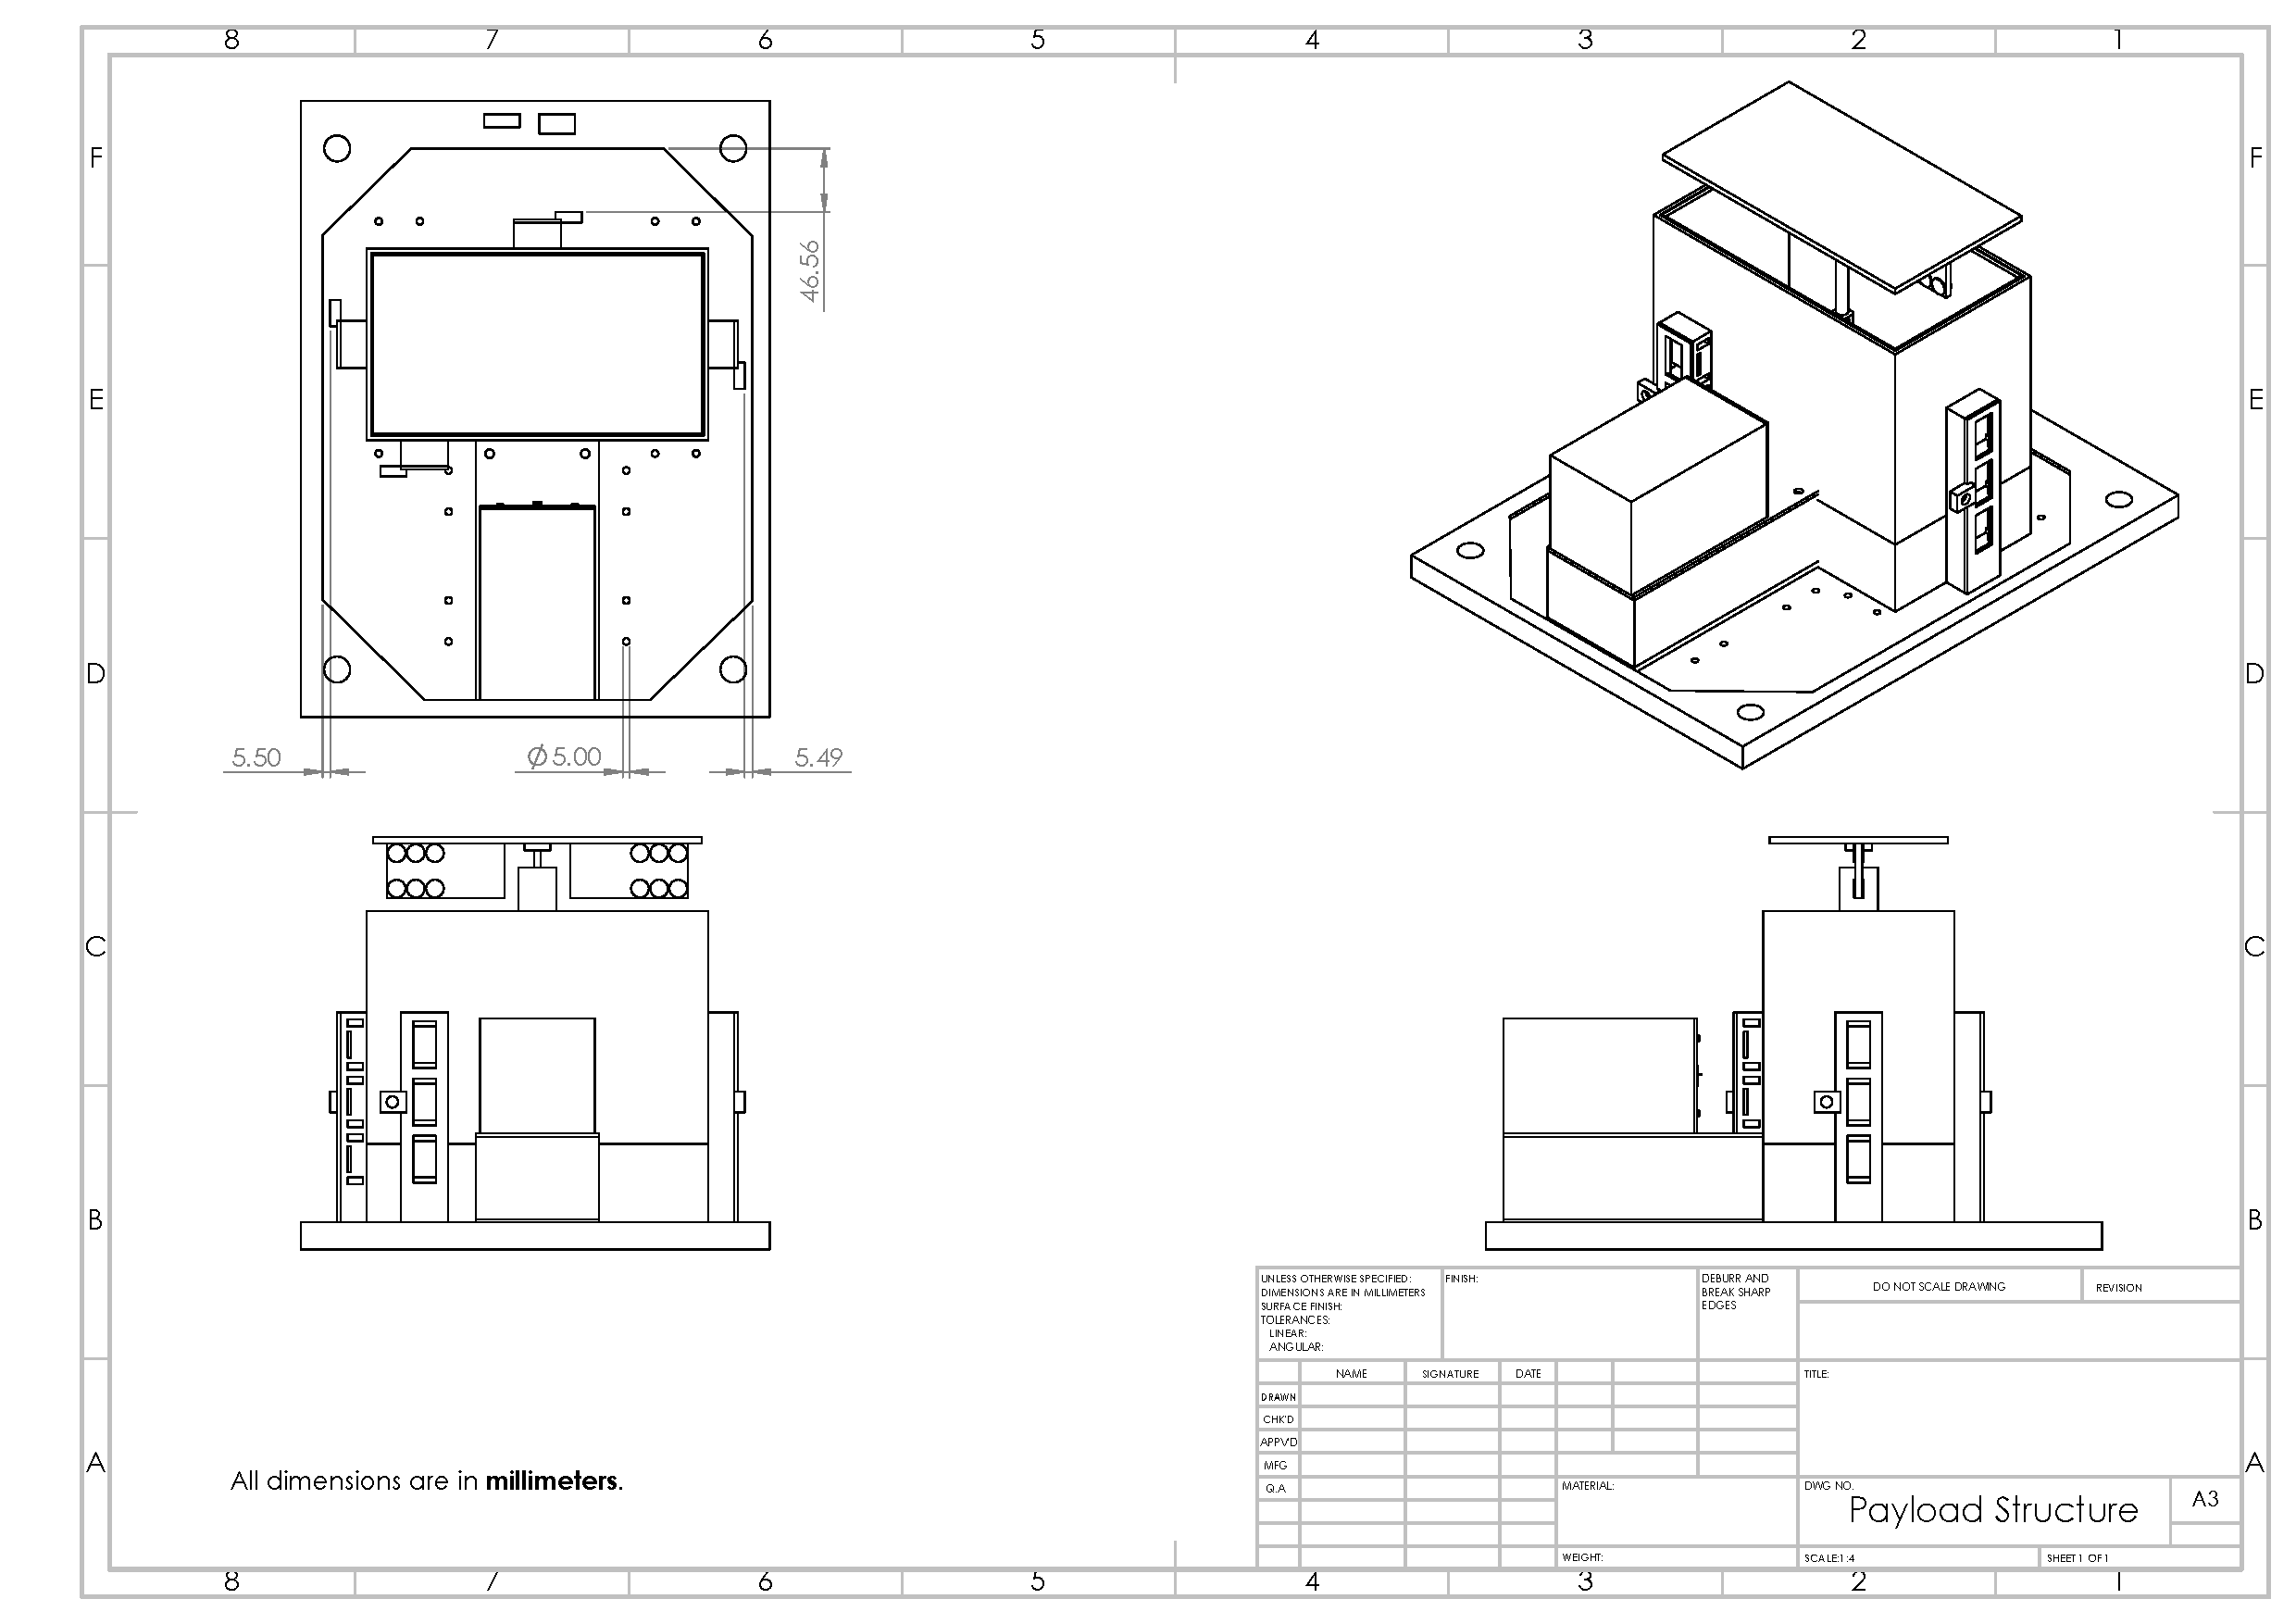
\includegraphics[width=\textwidth]{Figures/payload-structure-with-mount-holes.pdf}
    \caption{Drawing of the payload. The holes which will be drilled into the payload plate are shown. Each subsystem will be mounted to the plate with L-brackets. }
    \label{fig:payload-drawing}
  \end{figure}  
  \begin{figure}[H]
    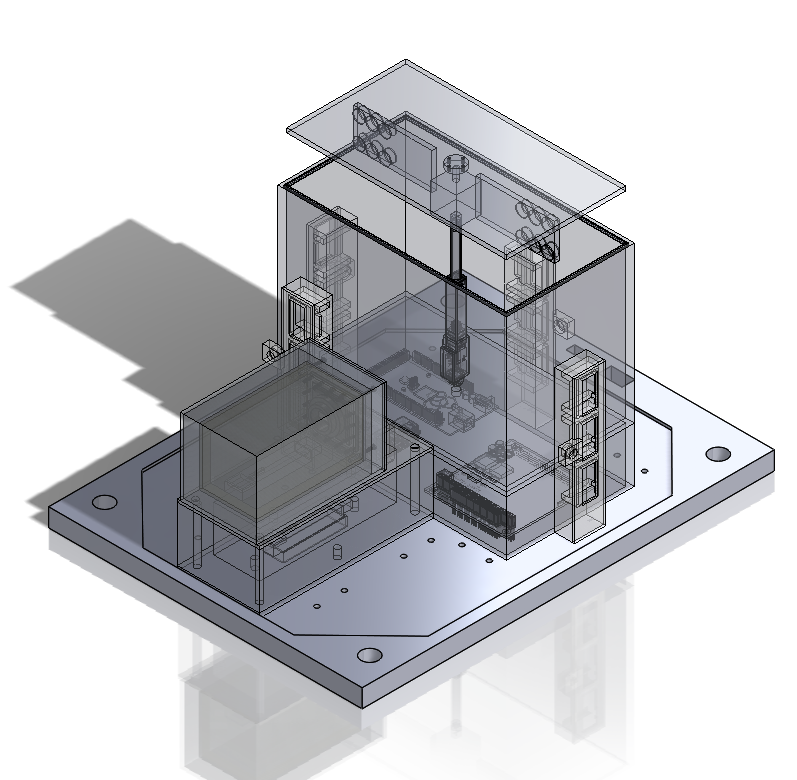
\includegraphics[width=\textwidth]{Figures/payload-transparent.png}
    \caption{Isometric, transparent view of the payload.}
    \label{fig:payload-transparent}
  \end{figure}  
  
  % Astrobio-electronics system
  \begin{figure}[H]
    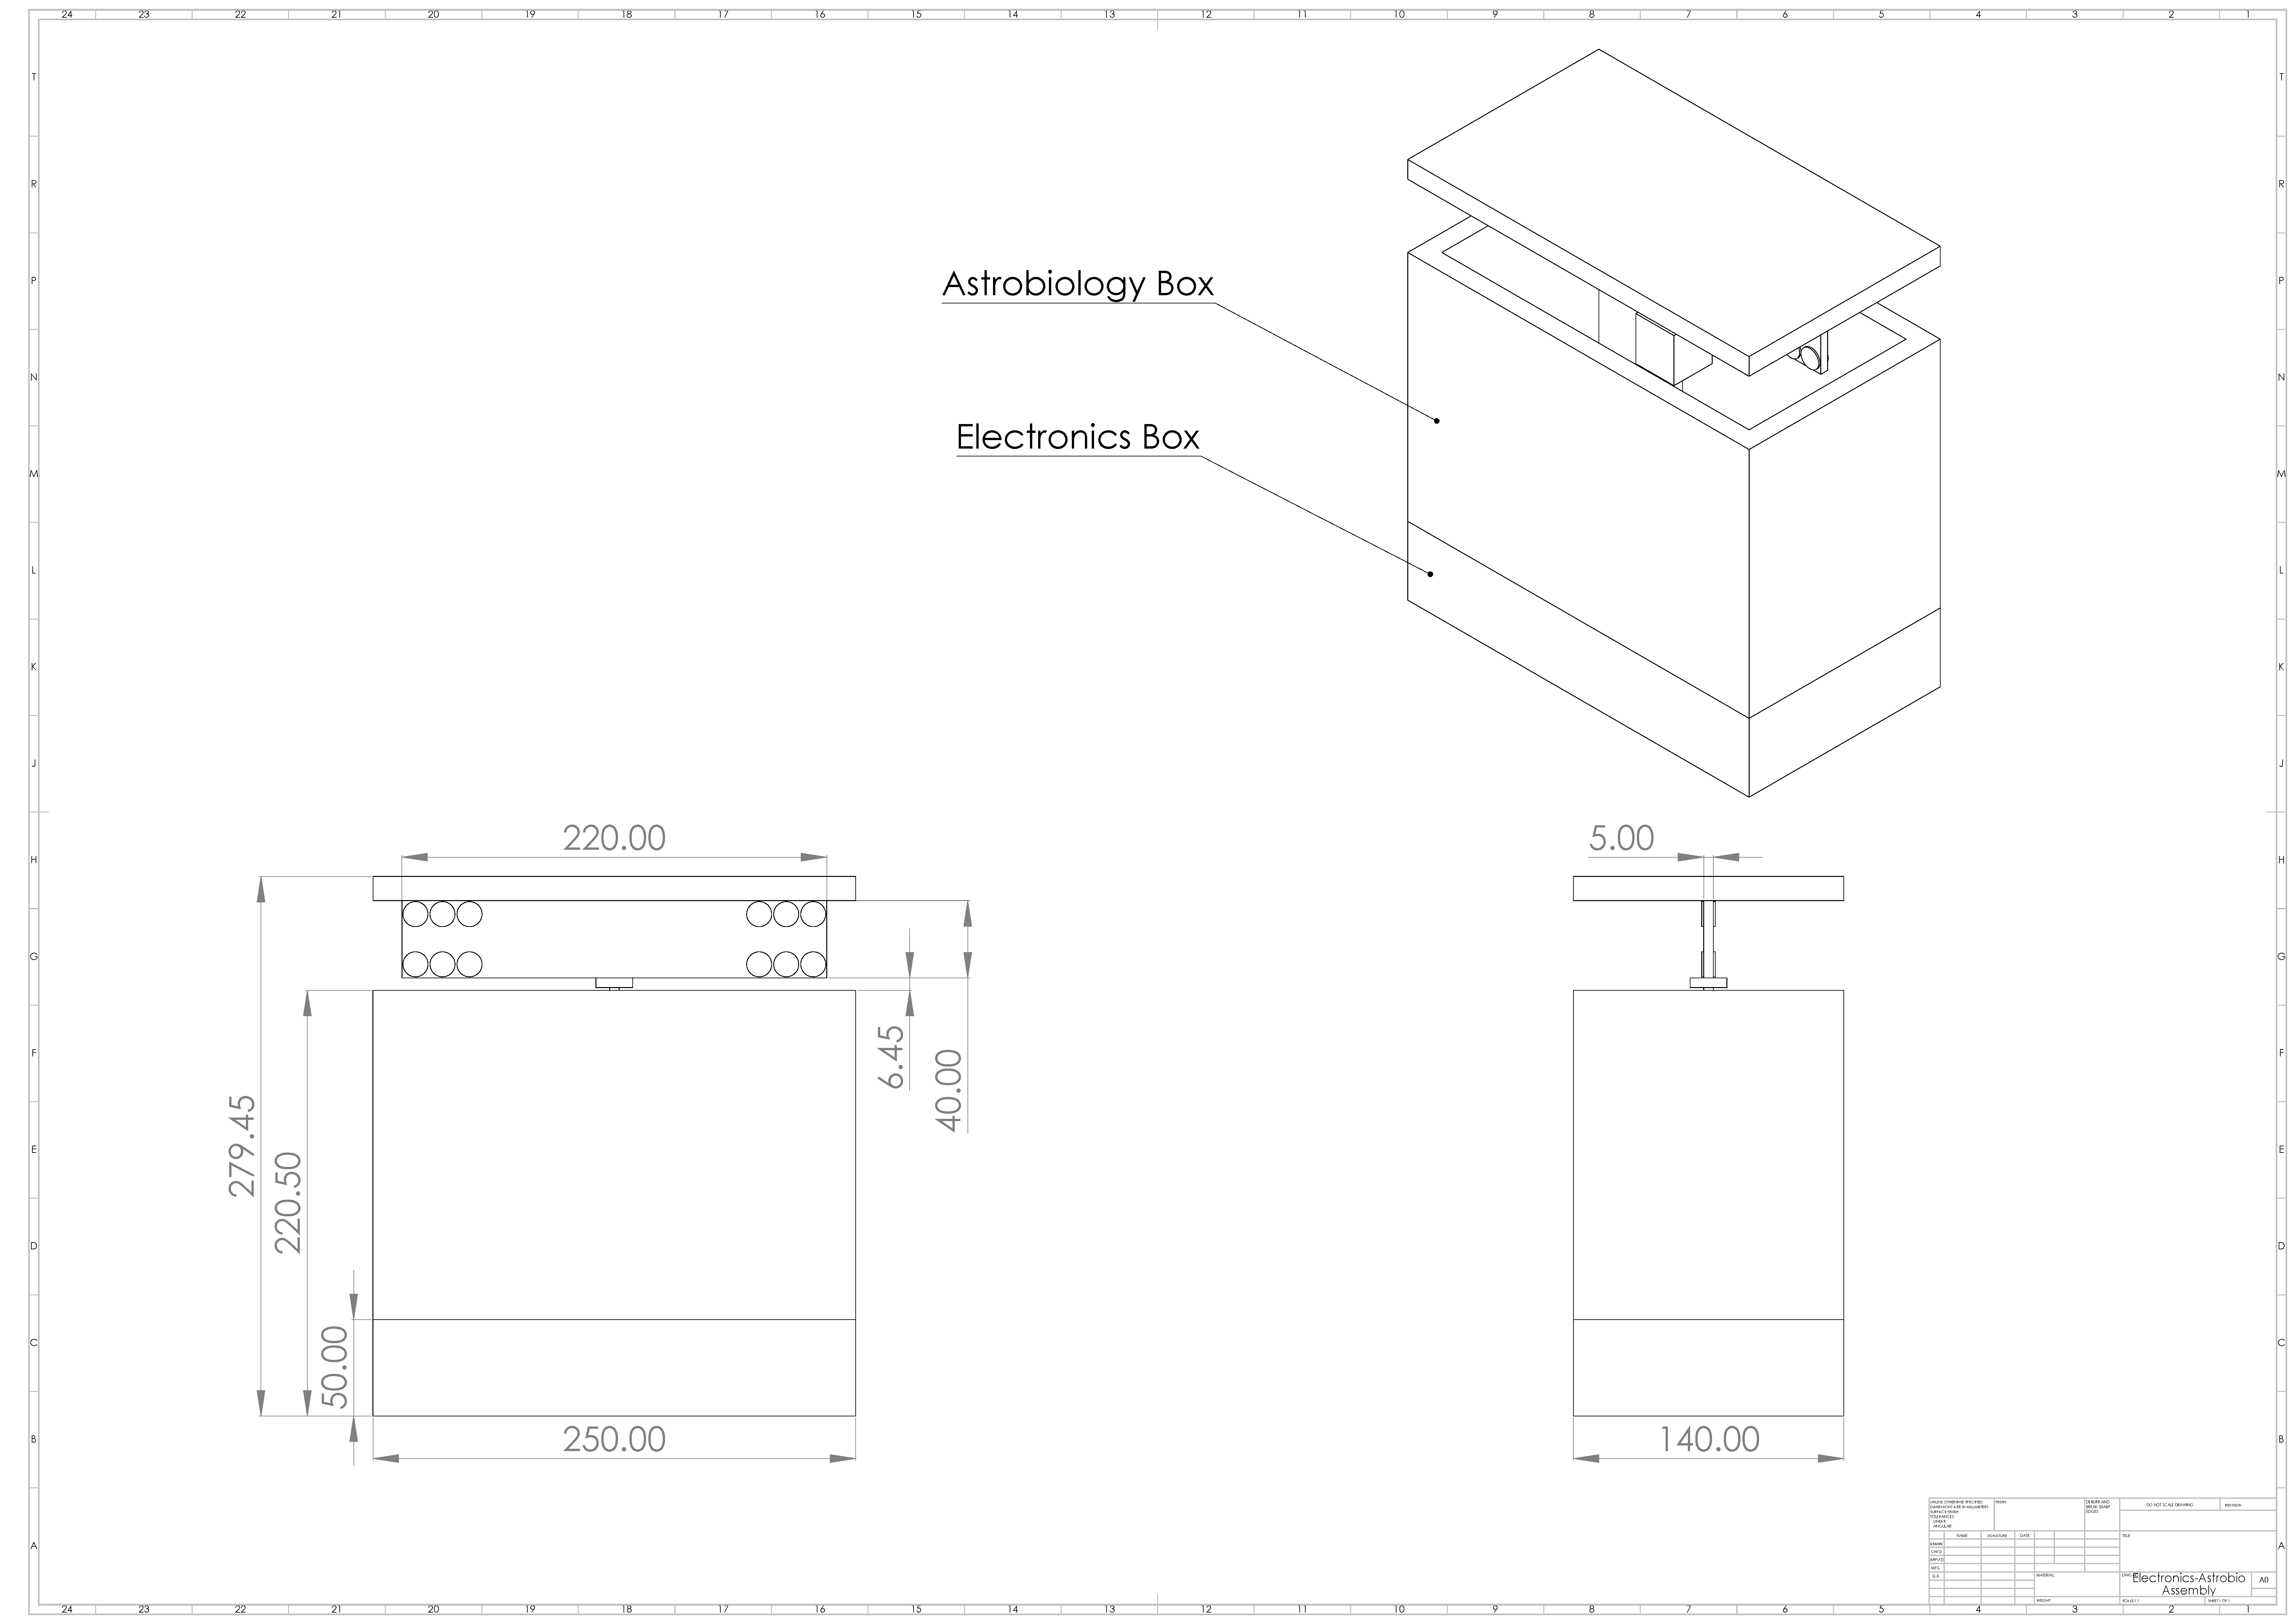
\includegraphics[width=\textwidth]{Figures/astrobio-electronics.pdf}
    \caption{Drawing of the deployed astrobiology system.}
    \label{fig:astrobio-electronics-drawing}
  \end{figure}
  \begin{figure}[H]
    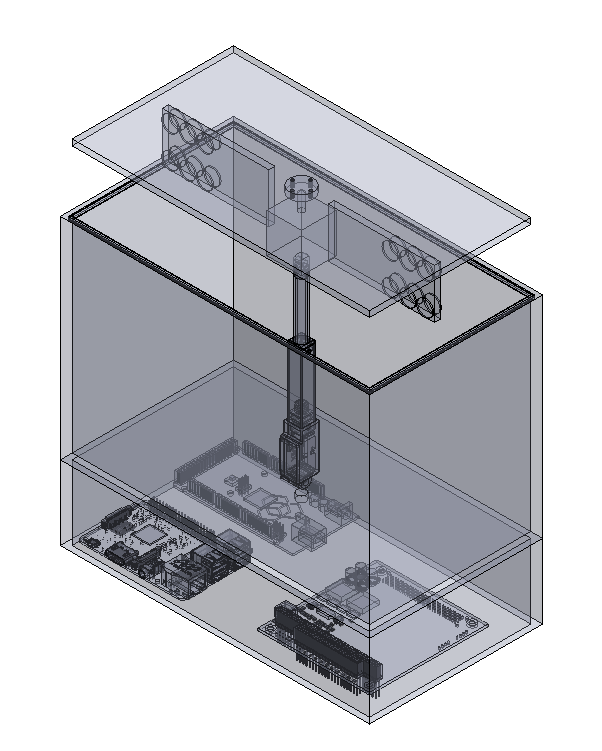
\includegraphics[width=\textwidth]{Figures/astrobio-electronics-deployed-transparent.png}
    \caption{Isometric, transparent view of the deployed astrobiology and electronics systems. All electronic components can be seen inside.}
    \label{fig:astrobio-electronics-image}
  \end{figure}
  \begin{figure}[H]
    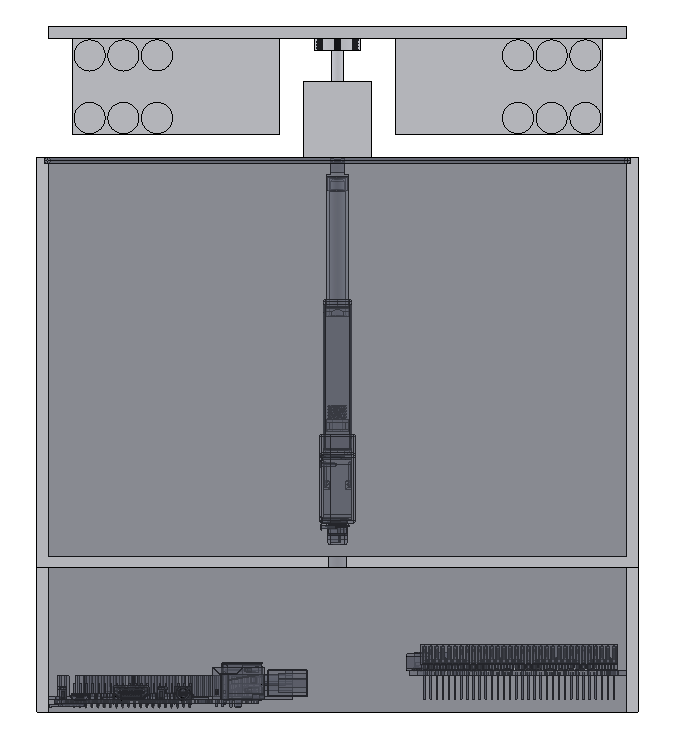
\includegraphics[width=\textwidth]{Figures/astrobio-electronics-deployed-transparent-sideview.png}
    \caption{Transparent Side view of the astrobiology and electronics box.}
    \label{fig:astrobio-electronics-image-sideview}
  \end{figure}
  \begin{figure}[H]
    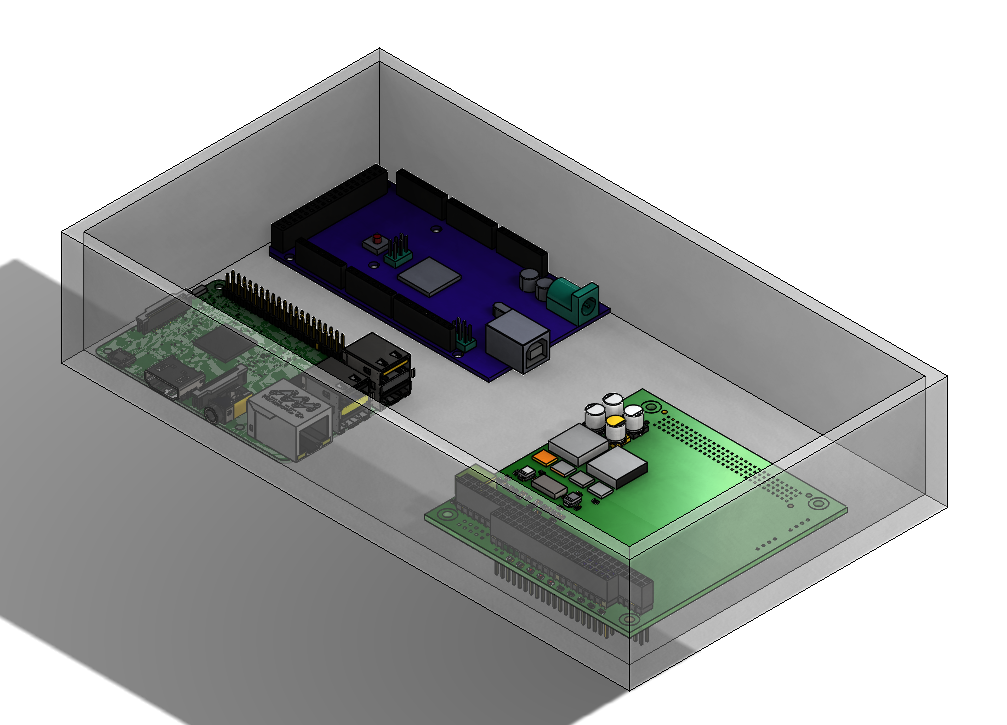
\includegraphics[width=\textwidth]{Figures/electronics-box.png}
    \caption{Layout of the electronics box.}
    \label{fig:electronics-box}
  \end{figure}  

    \begin{figure}[H]
    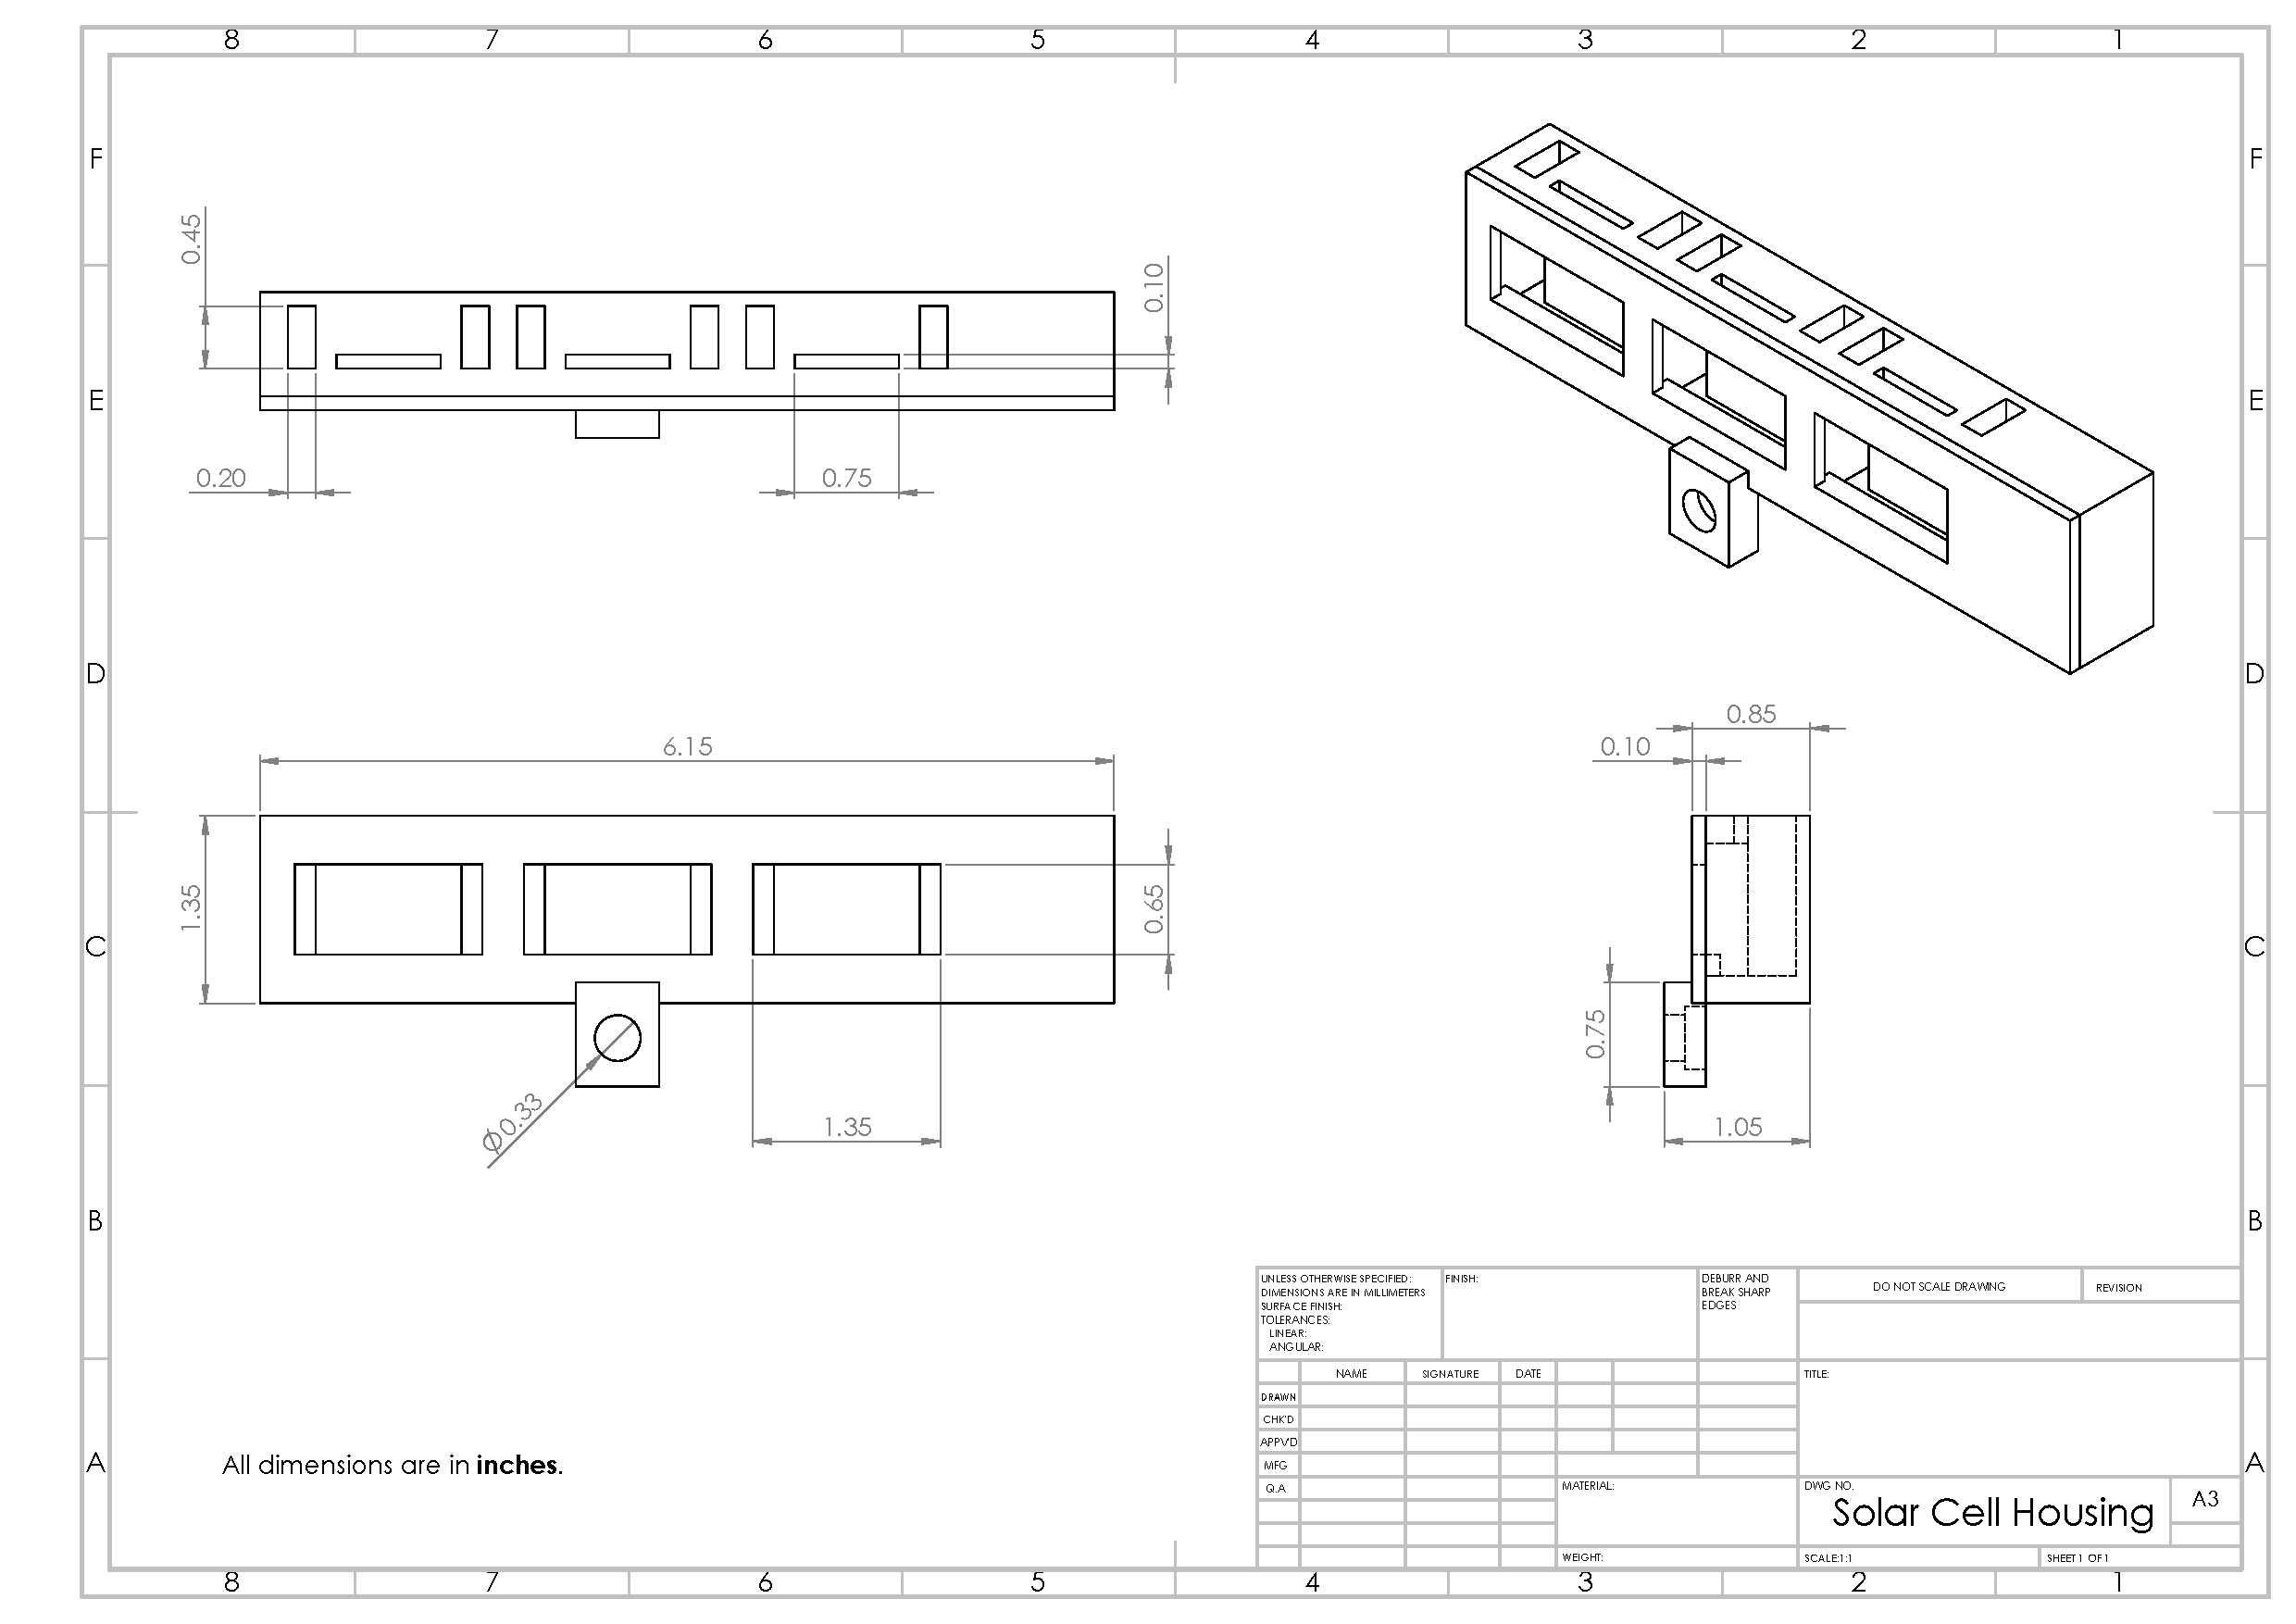
\includegraphics[width=\textwidth]{Figures/solar-cell-housing.pdf}
    \caption{Drawing of the solar cell housing.}
    \label{fig:solar-cell-housing}
  \end{figure}  


  % Unpressurized MiniPIX case
  \begin{figure}[H]
    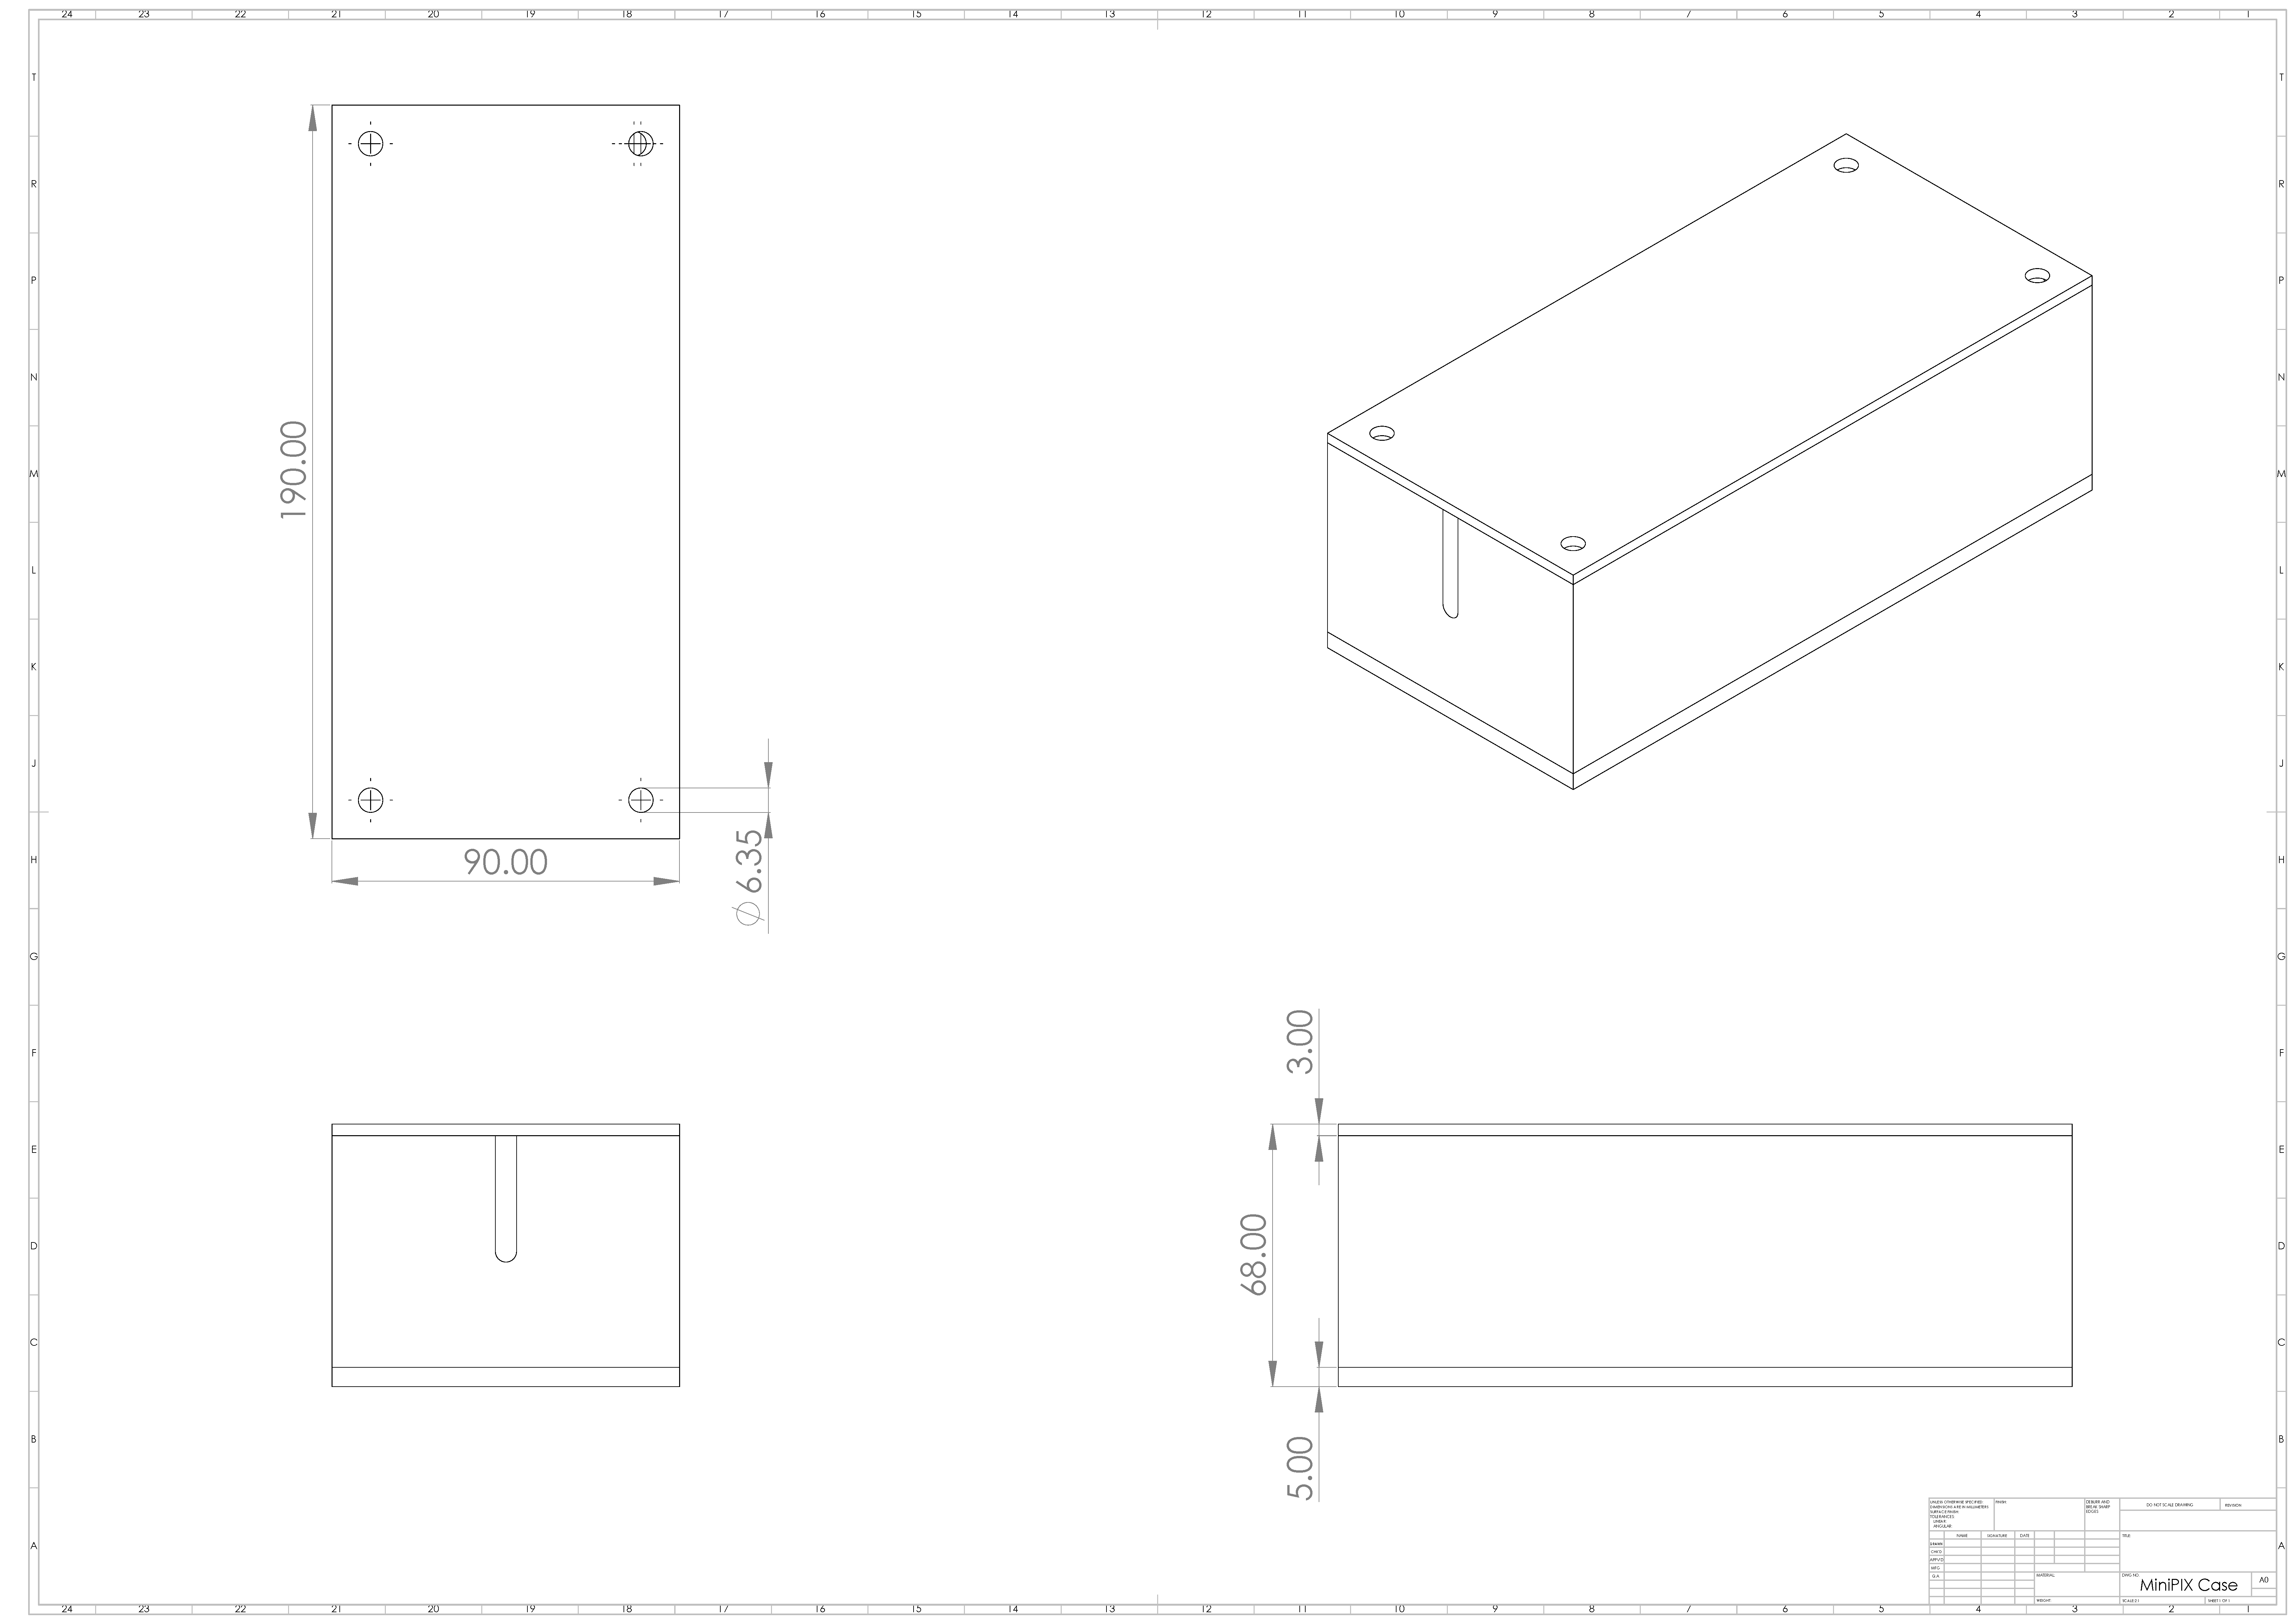
\includegraphics[width=\textwidth]{Figures/minipix-case.pdf}
    \caption{Drawing of the unpressurized MiniPIX case.}
    \label{fig:minipix-case-drawing}
  \end{figure}  
  \begin{figure}[H]
    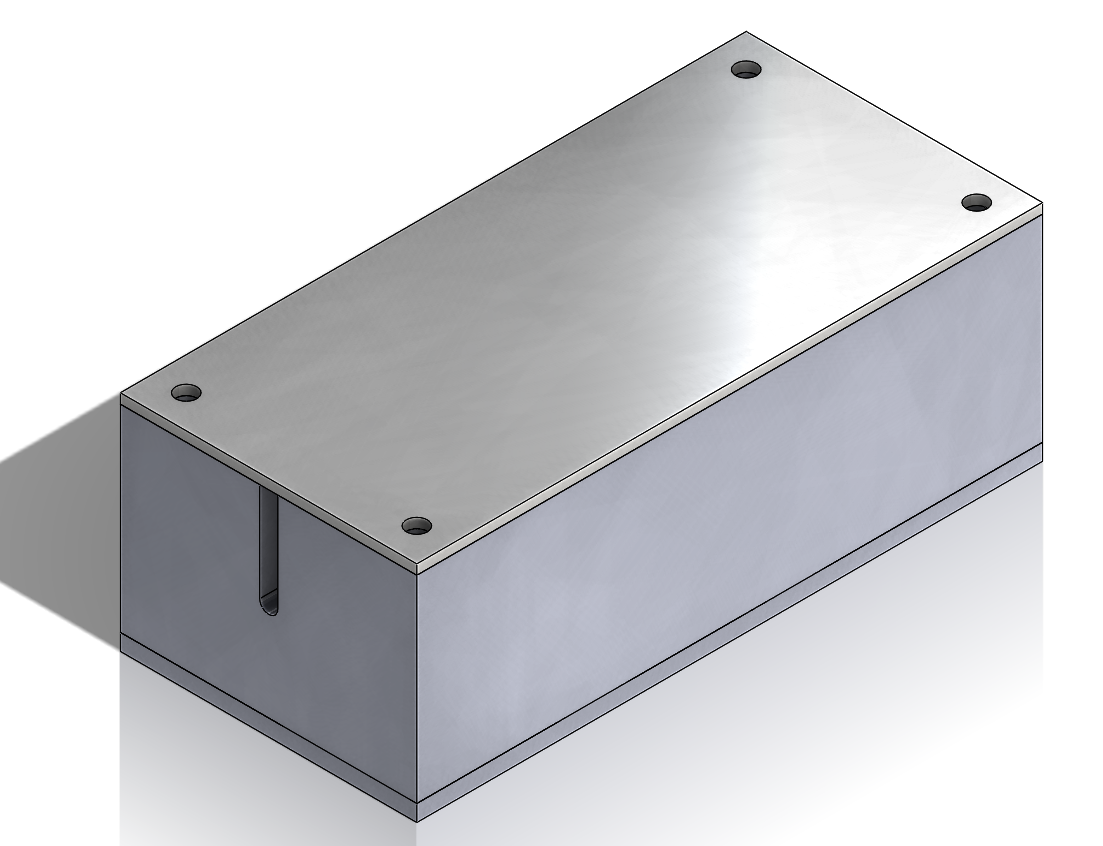
\includegraphics[width=\textwidth]{Figures/minipix-case-closed.png}
    \caption{Isometric view of the unpressurized MiniPIX case.}
    \label{fig:minipix-case-closed-image}
  \end{figure}
  \begin{figure}[H]
    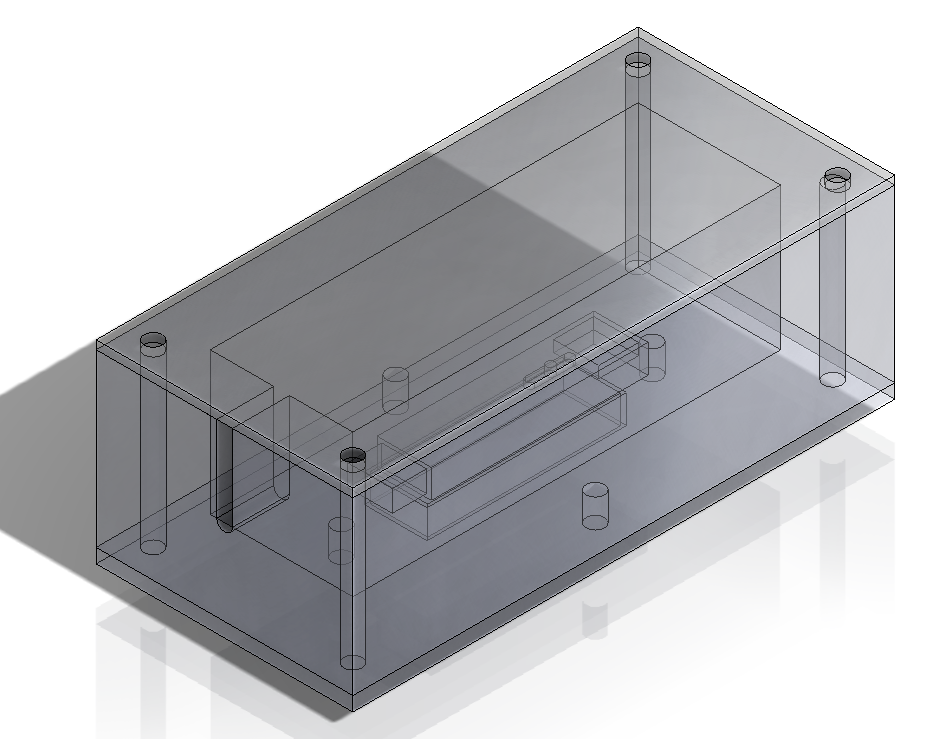
\includegraphics[width=\textwidth]{Figures/minipix-case-transparent.png}
    \caption{Isometric,transparent view of the unpressurized MiniPIX case.}
    \label{fig:minipix-case-closed-transparent-image}
  \end{figure}  
  \begin{figure}[H]
    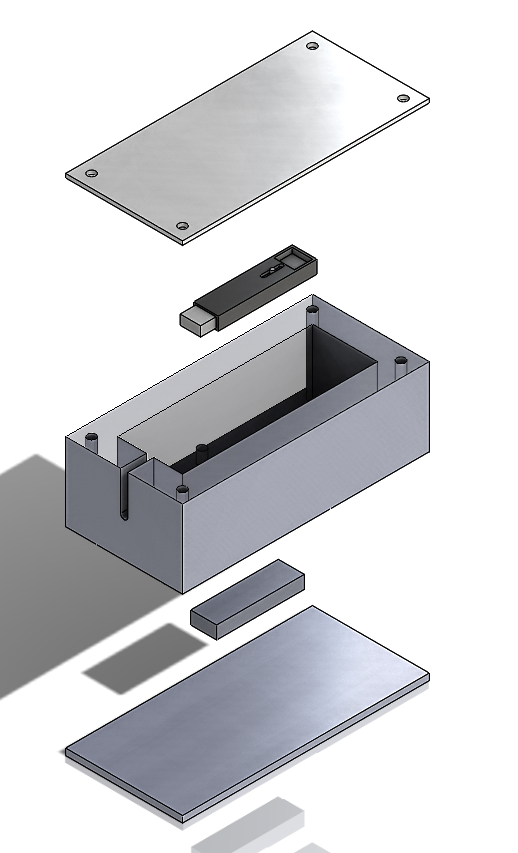
\includegraphics[width=0.7\textwidth]{Figures/minipix-case-exploded.png}
    \caption{Exploded view of the unpressurized MiniPIX case.}
    \label{fig:minipix-case-exploded-image}
  \end{figure}  
  
  % ISS system
  \begin{figure}[H]
    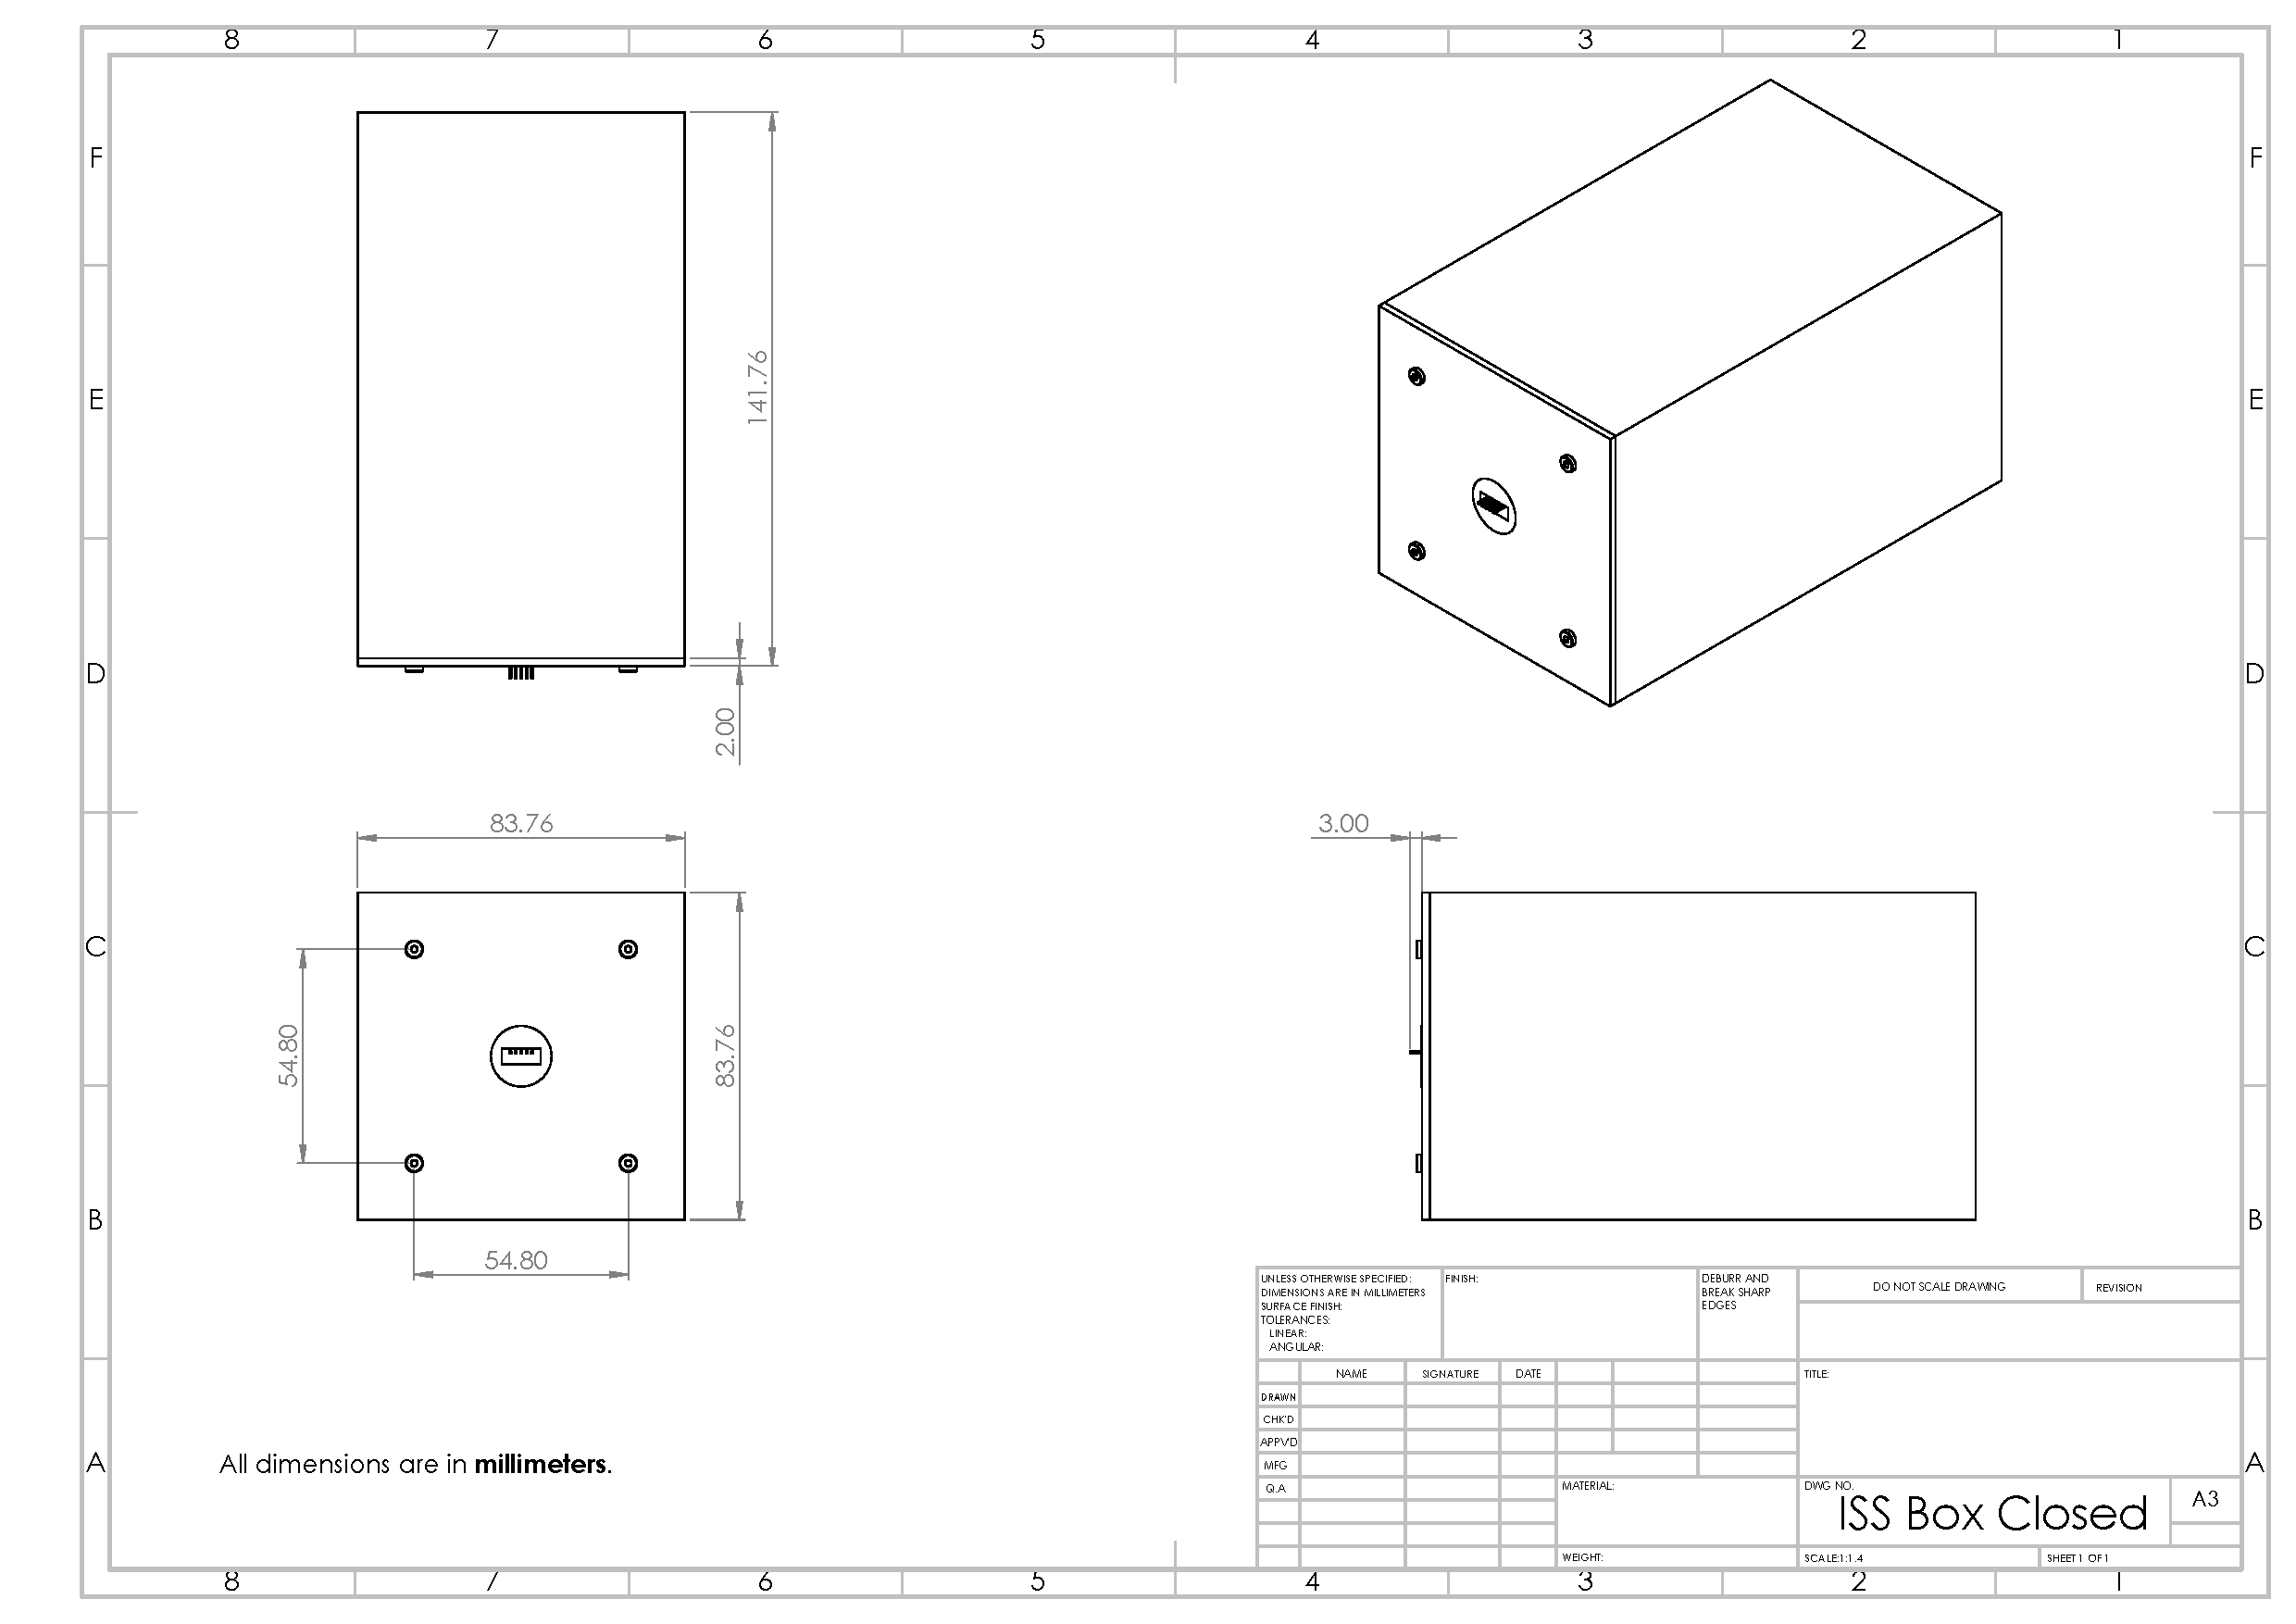
\includegraphics[width=\textwidth]{Figures/iss-closed.pdf}
    \caption{Drawing of the closed ISS module.}
    \label{fig:iss-closed-drawing}
  \end{figure}
  \begin{figure}[H]
    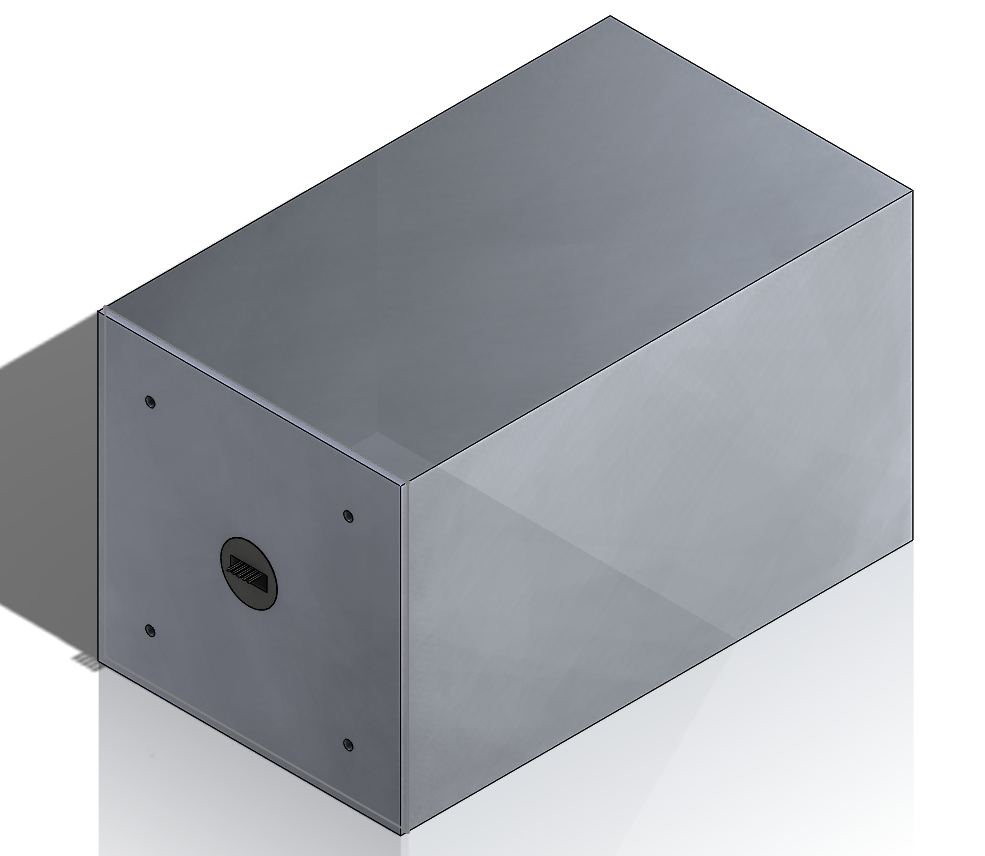
\includegraphics[width=\textwidth]{Figures/iss-closed.png}
    \caption{Isometric view of the closed ISS module.}
    \label{fig:iss-closed-image}
  \end{figure}
  \begin{figure}[H]
    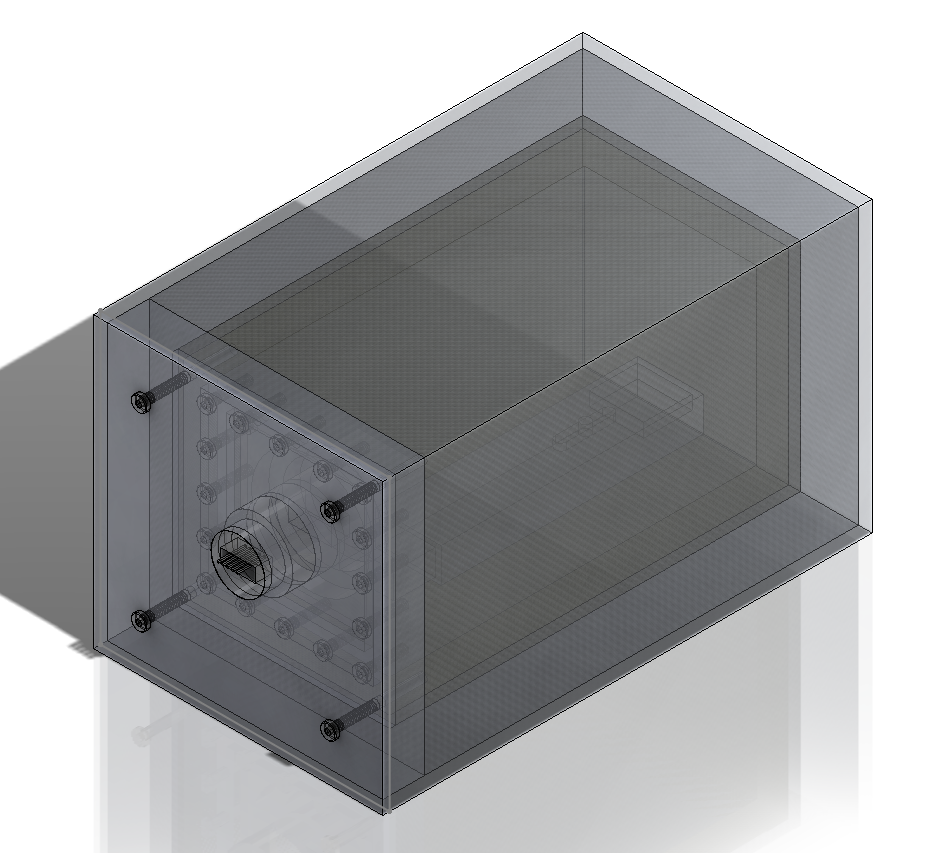
\includegraphics[width=\textwidth]{Figures/iss-closed-transparent.png}
    \caption{Isometric, transparent view of the closed ISS module.}
    \label{fig:iss-closed-transparent-image}
  \end{figure}
  \begin{figure}[H]
    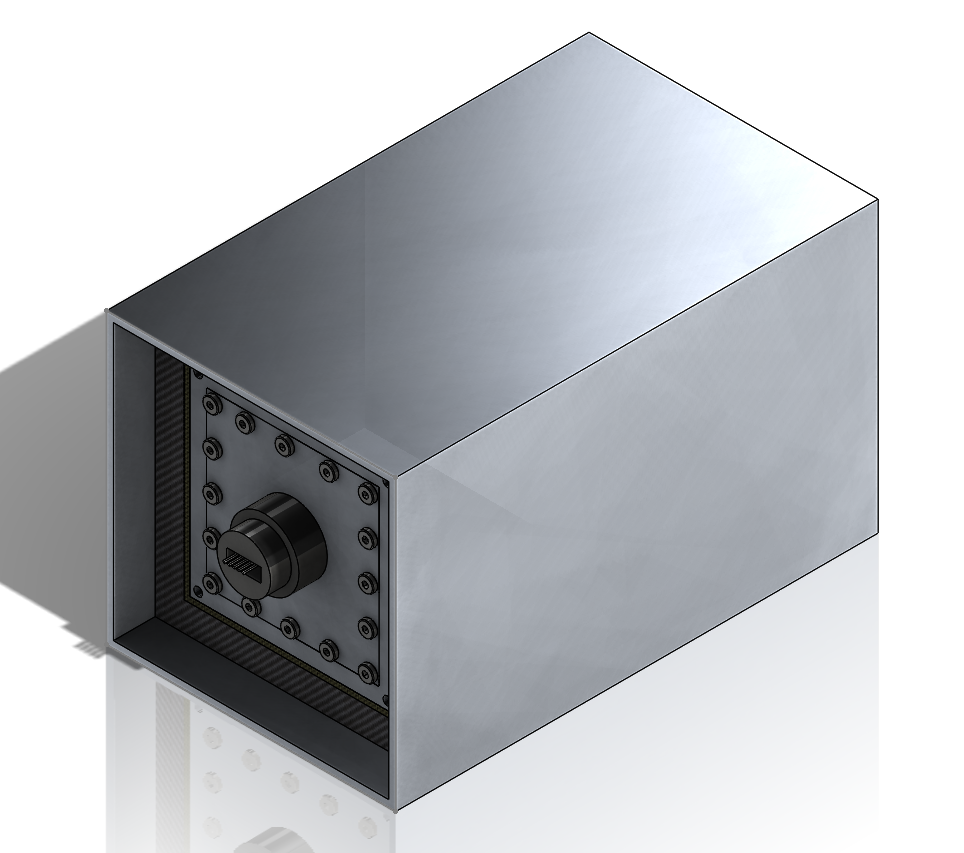
\includegraphics[width=\textwidth]{Figures/iss.png}
    \caption{Isometric view of the ISS showing the casing of the pressurized inner container.}
    \label{fig:iss-image}
  \end{figure}
  \begin{figure}[H]
    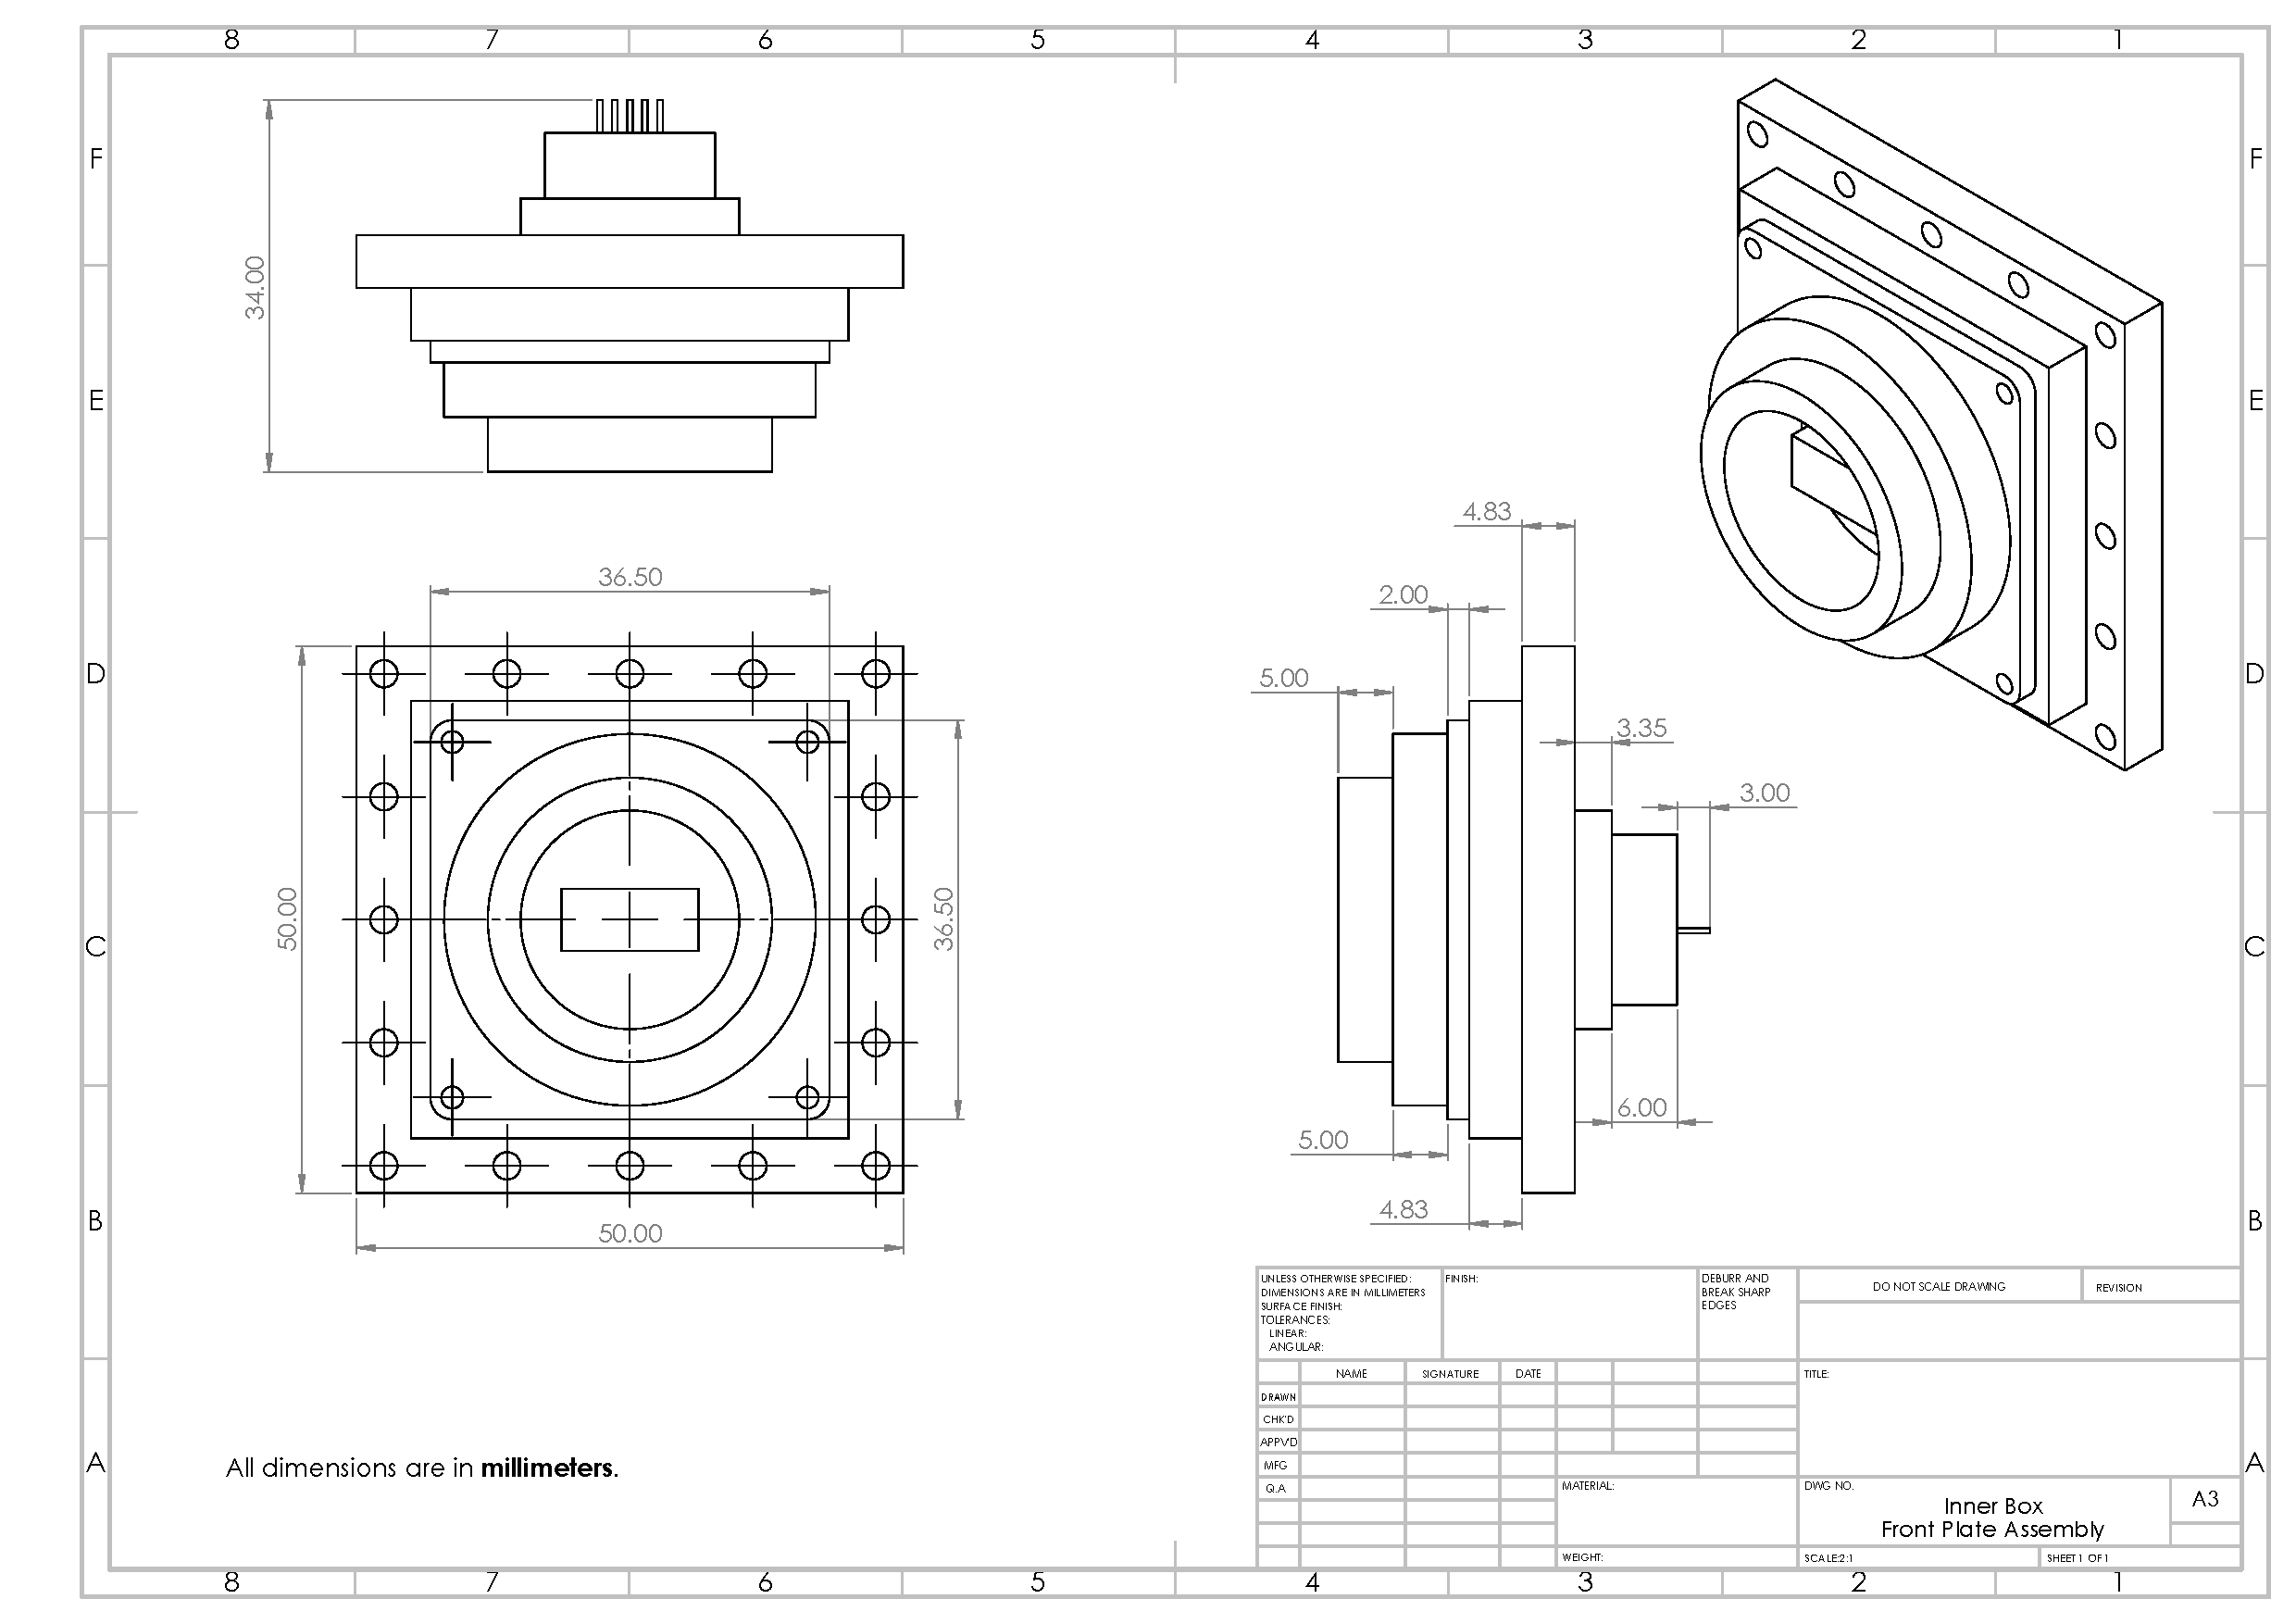
\includegraphics[width=\textwidth]{Figures/front-plate-assembly-with-feedthrough.pdf}
    \caption{Removable aluminum plate to contain the atmosphere within the ISS module.}
    \label{fig:InnerAluminumPlate}
  \end{figure}
  \begin{figure}[H]
    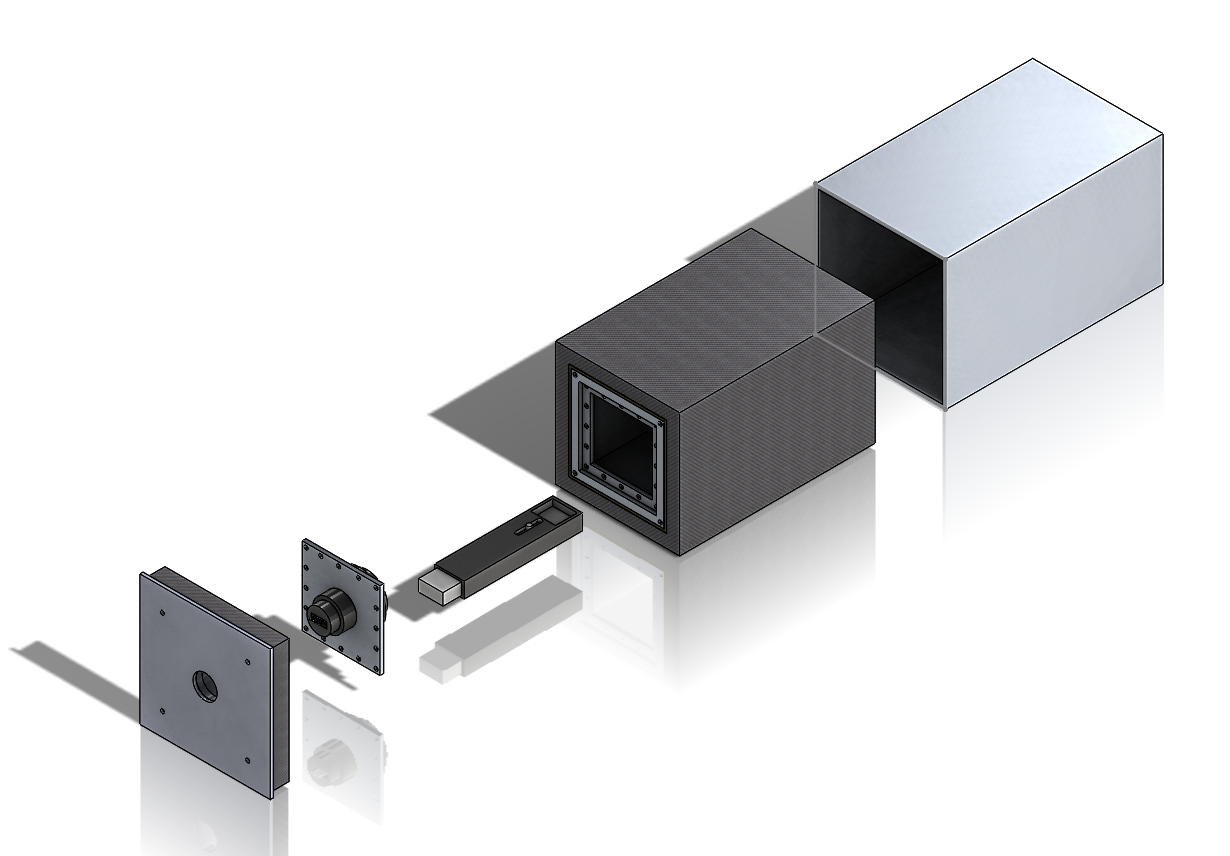
\includegraphics[width=\textwidth]{Figures/iss-exploded.png}
    \caption{Exploded view of the ISS module. From left to right: outer shell plate, hermetically sealed inner shell plate, MiniPIX, inner shell, outer shell.}
    \label{fig:iss-exploded-image}
  \end{figure}  

\end{centering}
